\documentclass{article}

%%%%
% PLOTS mapas y conglomerados
%%%%


\usepackage[utf8]{inputenc}
\usepackage{longtable}
\usepackage{authblk}
\usepackage{adjustbox}
\usepackage{natbib}


\title{LOS INDICES EN COLOMBIA}
% autores
\renewcommand\Authand{, y }
\author[1]{\normalsize Henry D Saenz}
\author[2]{\normalsize Laura M Montoya}

\affil[1,2]{\small  Universidad de los Andes\\
\texttt{{hd.saenz10,lm.montoya10}@uniandes.edu.col}}
\affil[1,2]{\small Ecole des Mines de Nantes\\
\texttt{{hsaenz16,lmontoya16}@imt-atlantique.fr}}

\date{29 de Junio de 2018}

%%%%
\usepackage{Sweave}
\begin{document}
\Sconcordance{concordance:Proyecto_Final_Introduccion.tex:Proyecto_Final_Introduccion.Rnw:%
1 28 1 1 0 29 1}


\maketitle


\begin{abstract}
Este es nuestro primer trabajo en exploraci<f3>n y modelamiento de <ed>ndices usando LATEX. Este trabajo lo he hecho bajo la filosof<ed>a de trabajo replicable. En este trabajo vamos a explorar
\end{abstract}

\section*{Introducci<f3>n}

Colombia, oficialmente Rep<fa>blica de Colombia, es un pa<ed>s soberano situado en la regi<f3>n noroccidental de Am<e9>rica del Sur, que se constituye en un estado unitario, social y democr<e1>tico de derecho cuya forma de gobierno es presidencialista. Es una rep<fa>blica organizada pol<ed>ticamente en 32 departamentos descentralizados y el Distrito capital de Bogot<e1>, sede del gobierno nacional.  En este trabajo vamos a estudiar el Indice de Desarrollo Humano en cado uno de los departamentos del pa<ed>s. 
El <ed>ndice de desarrollo humano (IDH) es un indicador del desarrollo humano por pa<ed>s, elaborado por el Programa de las Naciones Unidas para el Desarrollo (PNUD). El <ed>ndice de Desarrollo Humano (IDH) es un indicador sint<e9>tico de los logros medios obtenidos en las dimensiones fundamentales del desarrollo humano, a saber, tener una vida larga y saludable, adquirir conocimientos y disfrutar de un nivel de vida digno. El IDH es la media aritm<e9>tica de los <ed>ndices normalizados de cada una de las tres dimensiones. En este estudio no tenemos el detalle de cada una de las dimensiones, solamente el IDH por departamento.

Comencemos viendo que hay en la seccion \ref{univariada} en la pagina \pageref{univariada}.

\clearpage



\section{Exploración Univariada}\label{univariada}

En esta sección exploro cada índice.Nos vamos a interesar en la población cabecera y la poblacion resto. 


No podemos hacer tabla de frecuencias, entonces sacamos solamente los estadisticos:

% Table created by stargazer v.5.2.2 by Marek Hlavac, Harvard University. E-mail: hlavac at fas.harvard.edu
% Date and time: Fri, Jun 29, 2018 - 7:58:48 PM
\begin{table}[!htbp] \centering 
  \caption{Medidas estadisticas} 
  \label{stats} 
\begin{tabular}{@{\extracolsep{5pt}}lccccc} 
\\[-1.8ex]\hline 
\hline \\[-1.8ex] 
Statistic & \multicolumn{1}{c}{N} & \multicolumn{1}{c}{Median} & \multicolumn{1}{c}{Mean} & \multicolumn{1}{c}{Min} & \multicolumn{1}{c}{Max} \\ 
\hline \\[-1.8ex] 
IDH & 32 & 0.804 & 0.802 & 0.691 & 0.879 \\ 
Población.Cabecera & 32 & 717,197 & 1,196,730.000 & 13,090 & 10,070,801 \\ 
Población.Resto & 32 & 268,111.5 & 360,590.300 & 21,926 & 1,428,858 \\ 
Población.Total & 32 & 1,028,429 & 1,557,320.000 & 43,446 & 10,985,285 \\ 
\hline \\[-1.8ex] 
\end{tabular} 
\end{table} 
\begin{figure}[h]
\centering
\begin{adjustbox}{width=13cm,height=9cm,clip,trim=0cm 0cm 0cm 0cm}
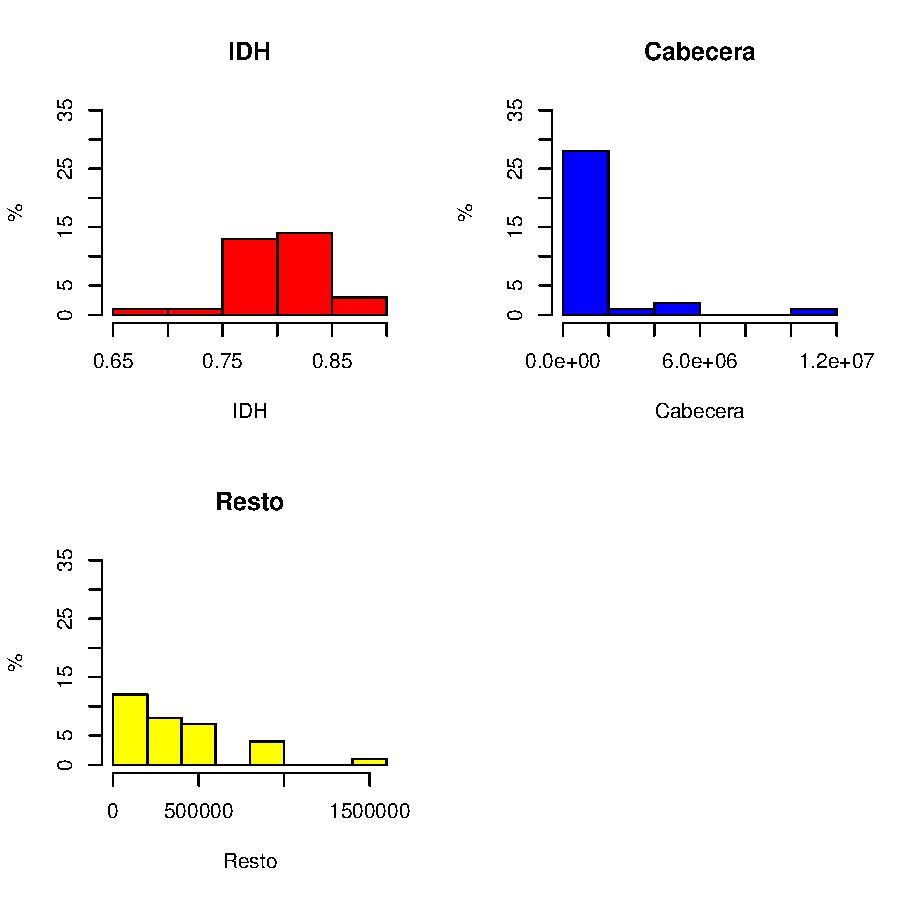
\includegraphics{Proyecto_Final_Univariada-corrPlotX}
\end{adjustbox}
\caption{correlacion entre predictores}
\label{corrPlotX}
\end{figure}

\clearpage

\endinput

\section{Exploracion Bivariada}\label{bivariada}

En este trabajo estamos interesados en el impacto de la poblacion en el IDH, veamos IDH con cada uno:


% Table created by stargazer v.5.2.2 by Marek Hlavac, Harvard University. E-mail: hlavac at fas.harvard.edu
% Date and time: Fri, Jun 29, 2018 - 5:58:25 PM
\begin{table}[!htbp] \centering 
  \caption{Correlacion del IDH con las demas variables} 
  \label{corrDem} 
\begin{tabular}{@{\extracolsep{5pt}} cc} 
\\[-1.8ex]\hline 
\hline \\[-1.8ex] 
cabeLog & restoLog \\ 
\hline \\[-1.8ex] 
$0.487$ & $0.177$ \\ 
\hline \\[-1.8ex] 
\end{tabular} 
\end{table} 

Veamos la correlacion entre las variables independientes:


% Table created by stargazer v.5.2.2 by Marek Hlavac, Harvard University. E-mail: hlavac at fas.harvard.edu
% Date and time: Fri, Jun 29, 2018 - 5:58:29 PM
\begin{table}[!htbp] \centering 
  \caption{Correlacion entre variables independientes} 
  \label{corrTableX} 
\begin{tabular}{@{\extracolsep{5pt}} ccc} 
\\[-1.8ex]\hline 
\hline \\[-1.8ex] 
 & cabeLog & restoLog \\ 
\hline \\[-1.8ex] 
cabeLog & 1 &  \\ 
restoLog & 0.84 & 1 \\ 
\hline \\[-1.8ex] 
\end{tabular} 
\end{table} 
Lo visto en la Tabla \ref{corrTableX} se refuerza claramente en la Figura \ref{corrPlotX}.

\begin{figure}
\centering
\begin{adjustbox}{width=7cm,height=7cm,clip,trim=1.5cm 0.5cm 0cm 1.5cm}
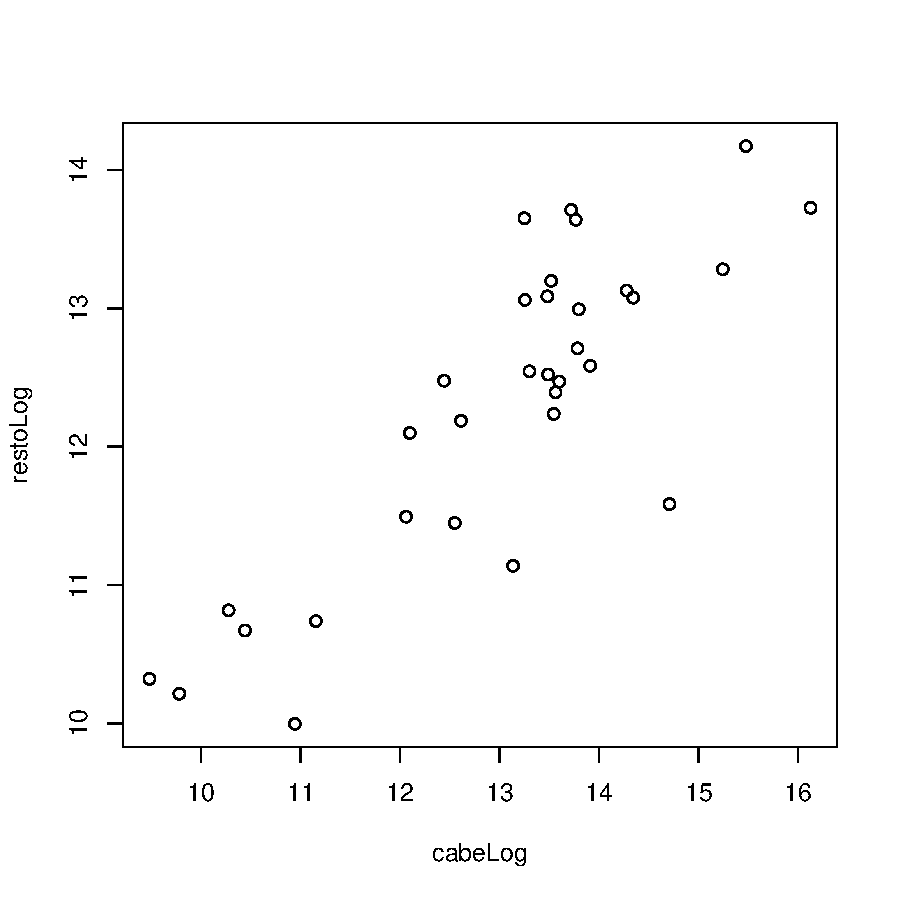
\includegraphics{Proyecto_Final_bivariada-corrPlotX}
\end{adjustbox}
\caption{correlacion entre predictores}
\label{corrPlotX}
\end{figure}
\endinput

\section{Modelos de Regresion}

Finalmente, vemos los modelos propuestos. Primero sin poblacion resto, luego con esa: Los resultados se muestran en la Tabla \ref{regresiones} de la pagina \pageref{regresiones}.

  
  
  
% Table created by stargazer v.5.2.2 by Marek Hlavac, Harvard University. E-mail: hlavac at fas.harvard.edu
% Date and time: Fri, Jun 29, 2018 - 8:11:13 PM
\begin{table}[!htbp] \centering 
  \caption{Modelos de Regresion} 
  \label{regresiones} 
\begin{tabular}{@{\extracolsep{5pt}}lcc} 
\\[-1.8ex]\hline 
\hline \\[-1.8ex] 
 & \multicolumn{2}{c}{\textit{Dependent variable:}} \\ 
\cline{2-3} 
\\[-1.8ex] & \multicolumn{2}{c}{IDH} \\ 
\\[-1.8ex] & (1) & (2)\\ 
\hline \\[-1.8ex] 
 cabeLog & 0.013$^{***}$ & 0.031$^{***}$ \\ 
  & (0.004) & (0.007) \\ 
  & & \\ 
 restoLog &  & $-$0.030$^{***}$ \\ 
  &  & (0.010) \\ 
  & & \\ 
 Constant & 0.634$^{***}$ & 0.766$^{***}$ \\ 
  & (0.055) & (0.065) \\ 
  & & \\ 
\hline \\[-1.8ex] 
Observations & 32 & 32 \\ 
R$^{2}$ & 0.238 & 0.425 \\ 
Adjusted R$^{2}$ & 0.212 & 0.385 \\ 
Residual Std. Error & 0.037 (df = 30) & 0.033 (df = 29) \\ 
F Statistic & 9.347$^{***}$ (df = 1; 30) & 10.706$^{***}$ (df = 2; 29) \\ 
\hline 
\hline \\[-1.8ex] 
\textit{Note:}  & \multicolumn{2}{r}{$^{*}$p$<$0.1; $^{**}$p$<$0.05; $^{***}$p$<$0.01} \\ 
\end{tabular} 
\end{table}   
  Como se vio en la Tabla \ref{regresiones}, cuando esta presente el \emph{indice de libertad mundial}, el \emph{Indice de libertad de prensa} pierde significancia.

\clearpage

\section{Exploracion Espacial}

Como acabamos de ver en la Tabla \ref{regresiones} en la pagina \pageref{regresiones}, si quisieras sintetizar la multidimensionalidad de nuestros indicadores, podramos usar tres de las cuatro variables que tenemos (un par de las originales tiene demasiada correlacion). 

%Asi, propongo que calculemos conglomerados de paises usando toda la informacion de tres de los indicadores. Como nuestras variables son ordinales utilizaremos un proceso de conglomeracion donde las distancia seran calculadas usando la medida {\bf gower} propuestas en \cite{gower_general_1971}, y para los enlazamientos usaremos la tecnica de {\bf medoides} segun \cite{reynolds_clustering_2006}. Los tres conglomerados se muestran en la Figura \ref{clustmap}.






\begin{figure}[h]
\centering
\begin{adjustbox}{width=18cm,height=14cm,clip,trim=25cm 0cm 0cm 0cm}
[1] 3 1 2  Group.1       IDH  cabeLog restoLog
1       1 0.8313529 14.03019 12.74569
2       2 0.7560000 13.05663 12.80485
3       3 0.7825714 10.58974 10.60684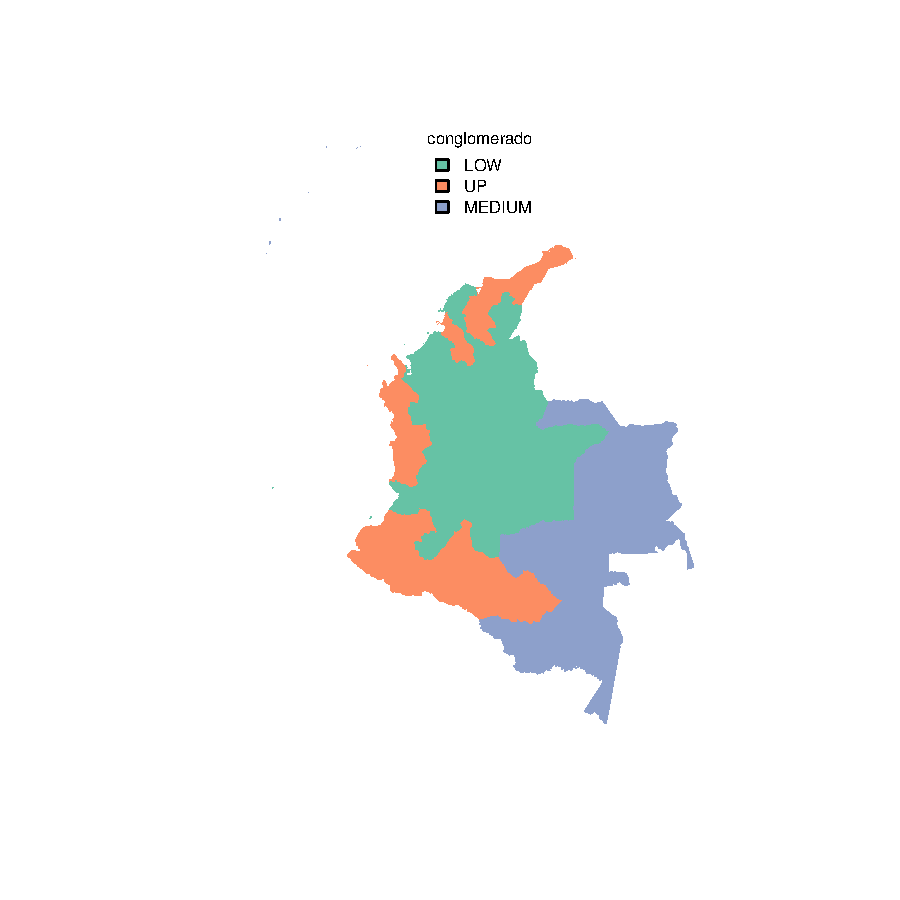
\includegraphics{Proyecto_Final_regresion-plotMapf}
\end{adjustbox}
\caption{Paises conglomerados segun sus indicadores sociopolaticos}\label{clustmap}
\end{figure}

\clearpage

\endinput



\bibliographystyle{apalike}
\renewcommand{\refname}{Bibliografia}
\bibliography{Colombia}

\end{document}
